\documentclass{article}
\usepackage{graphicx} % Required for inserting images
\usepackage{amsmath} 
\usepackage{float}

\title{ece6560}
\author{Pratiksha Pai}
\date{April 2024}

\begin{document}

\maketitle

\section{Problem Statement}

Image denoising is essential for enhancing the visual quality of digital images, which is vital for applications in fields such as medical imaging, remote sensing, and automated surveillance systems, where clarity and detail accuracy are crucial. We use Perona-Malik diffusion technique for its ability to preserve important edge details while effectively reducing noise, making it suitable for complex image processing tasks. In this study, we apply the Perona-Malik method under various conditions including different noise types like salt and pepper and Gaussian noise, different contrast levels like normal, high, and low contrast to evaluate its performance and robustness. Through these experiments, we aim to demonstrate the adaptability of the Perona-Malik technique across diverse scenarios and its potential to maintain integrity and enhance image usability in real-world applications.

\section{Mathematical Formulation}

Let us assume that the time-evolving image that we have is represented by \( I(x,y,t) \) where \( x \) and \( y \) are spatial co-ordinates, and \( t \) is the time variable. Now, we want to minimize the noise in the image. Let us focus on removing high-frequency noise such as salt and pepper or line drop noise for now. For penalizing high-frequency noise, we form an energy function that quantifies the gradient of the image. The intuition behind this is that as the image becomes smoother and smoother (de-noising), the gradient or the high-frequency components in the image decrease. Thus, the energy function that we are trying to minimize is given in equation (1)

\begin{align}
E(z) = \int C(z)dz
\end{align}

where \( z = \|\nabla I\| \) and \(\|\cdot\|\) is the L2 norm.

Now, this is the generic form of the energy function. An ideal de-noising would preserve the edges of the image while also smoothing the image. Thus, we want to smooth along the edges but not across them. For this purpose, we would formulate anisotropic diffusion called Perona Malik diffusion. The intuition is that the gradient at the edge would be large and should ideally be not diffused. Thus, the modification to the heat equation which diffuses homogeneously would be to add a variable diffusion coefficient. This diffusion coefficient is naturally a monotonically decreasing function of \( \nabla I \) which should be ideally 0 (no diffusion) at the edge and greater than zero at the non-edge parts of the image. The Perona-Malik anisotropic diffusion equation is given in equation(2)

\begin{align}
I_t = \nabla \cdot(F(\|\nabla I\|)\nabla I)
\end{align}

where \( F(\cdot) \) is the diffusion coefficient. Note: In literature, the diffusion coefficient is usually denoted by \( C \) however to avoid confusion with equation(1) I have denoted it by \( F \).

In [1], two diffusion coefficients functions are proposed:

\begin{align}
F(\|\nabla I\|) = \frac{1}{1 + \left(\frac{\|\nabla I\|}{K}\right)^2}
\end{align}

and

\begin{align}
F(\|\nabla I\|) = e^{-\left(\frac{\|\nabla I\|}{K}\right)^2}
\end{align}

\section{Discretization \& Stability Analysis}

\subsection{Discretization}

In order to run computer algorithms, we will have to discretize the PDE given in equation (2). Let us now simplify equation (2)

\[
I_t = \nabla \cdot (F(\|\nabla I\|)\nabla I)
    = \nabla F(\|\nabla I\|) \cdot \nabla I + F(\|\nabla I\|)\Delta I \tag{5}
\]

Let $F = F(\|\nabla I\|)$ be a shorthand for simplicity,

\begin{align}
I_t &= \nabla F \cdot \nabla I + F \Delta I \\
    &= (F_x + F_y)(I_x + I_y) + F(I_{xx} + I_{yy}) \\
    &= F_{x}I_x + F_{y}I_y + F(I_{xx} + I_{yy}) \tag{6}
\end{align}

Now, let us split each addition term and simplify it separately. First by substituting $F$ as in equation (3).

\begin{align}
F_{x}I_x &= \frac{\partial F}{\partial x} I_x \\
         &= \frac{\partial}{\partial x} \left( \frac{1}{1 + \frac{I_x^2}{K^2}} \right) I_x \\
         &= \frac{-K^2}{K^2 + I_x^2 + I_y^2}(2I_xI_{xx} + 2I_xI_yI_{xy}) \tag{7}
\end{align}

Similarly, by symmetry, $F_{y}I_y$ is given below.

\begin{align}
F_{y}I_y &= \frac{\partial F}{\partial y} I_y \\
         &= \frac{\partial}{\partial y} \left( \frac{1}{1 + \frac{I_y^2}{K^2}} \right) I_y \\
         &= \frac{-K^2}{K^2 + I_x^2 + I_y^2}(2I_yI_{yy} + 2I_xI_yI_{xy}) \tag{8}
\end{align}

From equations (6,7,8)

\begin{align}
I_t &= (2I_x^2I_{xx} + 2I_xI_yI_{xy}) + (2I_y^2I_{yy} + 2I_xI_yI_{xy}) + (K^2 + I_x^2 + I_y^2)(I_{xx} + I_{yy}) \\
    &= (I_{xx} - I_{yy})(I_x^2 - I_y^2) + K^2(I_{xx} + I_{yy}) - 4I_xI_yI_{xy} \\
    &= \frac{K^2(I_{xx} + I_{yy}) - 2I_x^2I_{xx} - 2I_y^2I_{yy} - 4I_xI_yI_{xy}}{K^2 + I_x^2 + I_y^2} \tag{9}
\end{align}

Similarly, we substitute $F$ as in equation (4).

\begin{align}
F_{x}I_x &= \frac{\partial F}{\partial x} I_x \\
         &= \frac{\partial}{\partial x} \left( e^{-\frac{I_x^2 + I_y^2}{K^2}} \right) I_x \\
         &= e^{-\frac{I_x^2 + I_y^2}{K^2}} \left( -\frac{2I_x}{K^2}(2I_xI_{xx} + 2I_xI_yI_{xy}) \right) \tag{10}
\end{align}

Similarly, by symmetry, $F_{y}I_y$ is given below.

\begin{align}
F_{y}I_y &= \frac{\partial F}{\partial y} I_y \\
         &= \frac{\partial}{\partial y} \left( e^{-\frac{I_x^2 + I_y^2}{K^2}} \right) I_y \\
         &= e^{-\frac{I_x^2 + I_y^2}{K^2}} \left( -\frac{2I_y}{K^2}(2I_yI_{yy} + 2I_xI_yI_{xy}) \right) \tag{11}
\end{align}

From equations (6,9,10)

\begin{align}
I_t &= K^2(I_{xx} + I_{yy}) - 2I_x^2I_{xx} - 2I_y^2I_{yy} - 4I_xI_yI_{xy} \\
    &= \frac{K^2(I_{xx} + I_{yy}) - 2I_x^2I_{xx} - 2I_y^2I_{yy} - 4I_xI_yI_{xy}}{K^2(e^{\frac{I_x^2 + I_y^2}{K^2}})} \tag{12}
\end{align}

To code this in a program we now use the forward and central differences to discretize the partial derivatives. With just one previous time step needed to determine the present time step, the forward difference for time approximation has the advantages of being simple to use and computationally efficient. While to minimize error, the central difference to approximate space derivatives is used.

\begin{align}
I_t &= \frac{I(t + \Delta t) - I(t)}{\Delta t} \\
I_x &= \frac{I(x + \Delta x) - I(x - \Delta x)}{2\Delta x} \\
I_y &= \frac{I(y + \Delta y) - I(y - \Delta y)}{2\Delta y} \\
I_{xx} &= \frac{I(x + \Delta x) - 2I_x + I(x - \Delta x)}{\Delta x^2} \\
I_{yy} &= \frac{I(y + \Delta y) - 2I_y + I(y - \Delta y)}{\Delta y^2} \\
% I_{xy} &= \frac{I(x + \Delta x, y + \Delta y) + I(x - \Delta x, y - \Delta y) - I(x + \Delta x, y - \Delta y) - I(x - \Delta x, y + \Delta y)}{4\Delta x\Delta y} \tag{13}
I_{xy} =\ &\frac{1}{4\Delta x\Delta y}\big[I(x + \Delta x, y + \Delta y) + I(x - \Delta x, y - \Delta y) \nonumber \\
&- I(x + \Delta x, y - \Delta y) - I(x - \Delta x, y + \Delta y)\big] \tag{13}
\end{align}

\subsection{Stability Analysis}

I will now use the Perona - Malik scheme of discretization given in [1] for this project since doing it by equations (9, 12 and 13) will be too complicated. Also, this method of discretization is widely popular and proved to be stable. I will closely follow the literature [1] to write the code.

Let \(\Delta x\) and \(\Delta y\) be the spatial steps and \(\Delta t\) be the time step. Now, with \(\Delta x = \Delta y = 1\) the discretization of Perona - Malik equation is given by,

% \begin{align}
% I(x, y, t + 1) = I(x, y, t) + \Delta t [C_N \nabla_N I(x, y, t) + C_S \nabla_S I(x, y, t) + C_E \nabla_E I(x, y, t) + C_W \nabla_W I(x, y, t)]
% \end{align}

\begin{align}
I(x, y, t + 1) =\ &I(x, y, t) + \Delta t \big[C_N \nabla_N I(x, y, t) + C_S \nabla_S I(x, y, t) \nonumber \\
&+ C_E \nabla_E I(x, y, t) + C_W \nabla_W I(x, y, t)\big]
\end{align}


where,

\begin{align}
\nabla_N I(x, y, t) &= I(x - 1, y, t) - I(x, y, t) \\
\nabla_S I(x, y, t) &= I(x + 1, y, t) - I(x, y, t) \\
\nabla_E I(x, y, t) &= I(x, y + 1, t) - I(x, y, t) \\
\nabla_W I(x, y, t) &= I(x, y - 1, t) - I(x, y, t)
\end{align}

with \( 0 < \Delta t \leq \frac{1}{4} \) for the scheme to be stable.

An efficient method for determining the CFL condition that avoids the need to compute the 2D DFT of equations (13) is to first calculate the CFL condition for the 1D heat equation, and then extend it to the 2D case due to its symmetry. This approach simplifies the process and saves computational resources. For our case let us define \( F(\|\nabla I\|) = F \) which is the real-valued diffusivity coefficient. Now, the stability condition for the 1D heat equation \( I_t = F * I_{xx} \) as derived in class is \( \Delta t \leq \frac{(\Delta x)^2}{2F} \). Substituting \(\Delta x = \frac{\Delta x}{\sqrt{2}} \), we get the CFL condition for 2D case as

\begin{align}
\Delta t &\leq \frac{(\Delta x)^2}{4F} \\
\Delta t &\leq \frac{(\Delta y)^2}{4F}
\end{align}

Let \(\Delta x = \Delta y = 1\)

\begin{align}
\Delta t &\leq \frac{1}{4F}
\end{align}

Now, from Figures 2 and 3, we see that the diffusivity coefficient is bounded between 0 and 1, thus for any value of \( K \), \( F \) will be bounded by \( 0 \leq F \leq 1 \) and \( \Delta t \leq 0.25 \) will ensure the convergence of the scheme. The code for the update equation is given below.


\section{Error Calculation}
The following metrics will be used to compare the quality of the denoised images.

\subsection{Peak Signal-to-Noise Ratio}
The ratio between the power of the maximum possible image intensity across a volume and the power of the distorting noise and other errors. Where \( \hat{v} \) is the denoised volume, \( v \) is the target volume, \( \text{max}(v) \) is the largest entry in the target volume, and \( \text{MSE} \) is the mean square error. Higher values of PSNR indicate a better denoising.

\[
\text{PSNR}(\hat{v}, v) = 20 \log_{10} \left(\frac{\text{max}(v)}{\sqrt{\text{MSE}(\hat{v}, v)}}\right)
\]

\subsection{Mean Square Error}
MSE tends to favor smoothness over sharpness. The subtraction within is performed entry-wise. Lower MSE indicates a better denoising.

\[
\text{MSE}(\hat{v}, v) = \frac{1}{n} \sum_{i=1}^{n} (\hat{v}_i - v_i)^2
\]

\section{Experiments}

\subsection{Sensitivity of Diffusion Coefficient to the Gradient}

An experiment was conducted to analyze the sensitivity of the diffusion coefficient \( F \) to changes in the image gradient for different values of the parameter \( K \). For this purpose, a range of image gradients was simulated, and the corresponding diffusion coefficient values were computed using the diffusion functions \( F_1 \) and \( F_2 \) as defined in equations (3) and (4), respectively.

Plots were generated to visually demonstrate the effect of varying \( K \) on the diffusion coefficient. These plots serve to illustrate how the diffusion process is influenced by the parameter \( K \), especially at different gradient magnitudes. The diffusion coefficient versus gradient plots for both \( F_1 \) and \( F_2 \) are included, highlighting the dependency of the diffusion process on the parameter \( K \).

\begin{figure}[H]
    \centering
    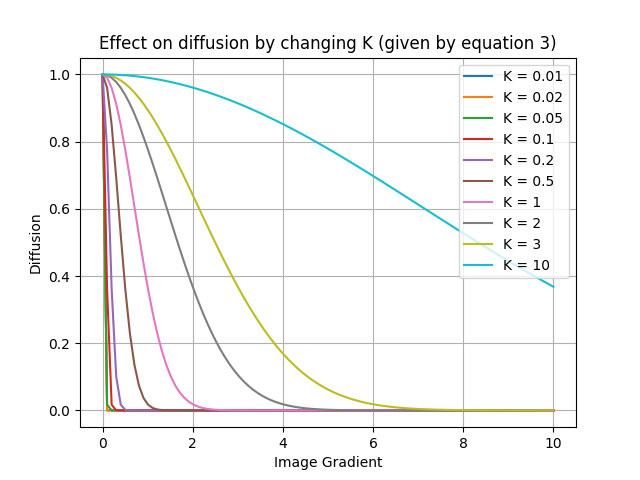
\includegraphics[width=0.8\textwidth]{plots/F1_equation_3.png}
    \caption{The sensitivity of the diffusion coefficient \( F_1 \) to the image gradient for different values of \( K \).}
    \label{fig:diffusion_f1}
\end{figure}

\begin{figure}[H]
    \centering
    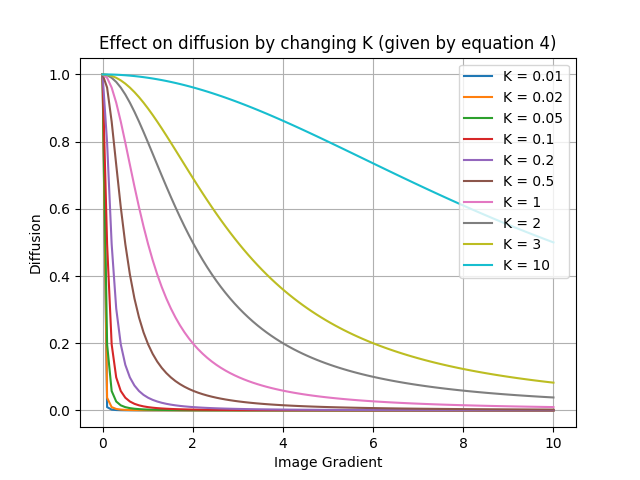
\includegraphics[width=0.8\textwidth]{plots/F2_equation_4.png}
    \caption{The sensitivity of the diffusion coefficient \( F_2 \) to the image gradient for different values of \( K \).}
    \label{fig:diffusion_f2}
\end{figure}

\subsection{PSNR Sensitivity Analysis}

A series of experiments were conducted to observe the sensitivity of the Peak Signal-to-Noise Ratio (PSNR) to the Perona-Malik diffusion parameters: the diffusion constant \( K \), the time step \( \Delta t \), and the number of iterations or steps. The denoising functions \( F_1 \) and \( F_2 \), defined by the diffusion equations, were applied to both Gaussian and salt-and-pepper noise affected images. The PSNR was computed against the original, undistorted image to gauge the quality of denoising.

For each parameter set, six scenarios were considered: three variations of \( K \), \( \Delta t \), and the number of steps for both types of noise. This comprehensive approach allowed for a detailed understanding of how each parameter influences the denoising performance as reflected by the PSNR values. Plots were generated to visualize the PSNR dependency on each parameter, providing insights into the optimal parameter selection for the Perona-Malik algorithm.

The results are presented in a series of figures showing the PSNR values for varying \( K \), \( \Delta t \), and the number of steps, with separate plots for the Gaussian noise and salt-and-pepper noise scenarios.

% Gauss Noise
\begin{figure}[H]
    \centering
    \includegraphics[width=0.8\textwidth]{plots/gaussian_psnr_varying_del_t.png}
    \caption{PSNR vs \( \Delta t \) for Gaussian Noise.}
    \label{fig:psnr_sensitivity_1}
\end{figure}

\begin{figure}[H]
    \centering
    \includegraphics[width=0.8\textwidth]{plots/gaussian_psnr_varying_k.png}
    \caption{PSNR vs \( K \) for Gaussian Noise.}
    \label{fig:psnr_sensitivity_2}
\end{figure}

\begin{figure}[H]
    \centering
    \includegraphics[width=0.8\textwidth]{plots/gaussian_psnr_varying_steps.png}
    \caption{PSNR vs Steps for Gaussian Noise.}
    \label{fig:psnr_sensitivity_3}
\end{figure}

% salt and pepper noise
\begin{figure}[H]
    \centering
    \includegraphics[width=0.8\textwidth]{plots/salt_pepper_psnr_varying_del_t.png}
    \caption{PSNR vs \( \Delta t \) for Gaussian Noise.}
    \label{fig:psnr_sensitivity_4}
\end{figure}

\begin{figure}[H]
    \centering
    \includegraphics[width=0.8\textwidth]{plots/salt_pepper_psnr_varying_k.png}
    \caption{PSNR vs \( K \) for Gaussian Noise.}
    \label{fig:psnr_sensitivity_5}
\end{figure}

\begin{figure}[H]
    \centering
    \includegraphics[width=0.8\textwidth]{plots/salt_pepper_psnr_varying_steps.png}
    \caption{PSNR vs Steps for Gaussian Noise.}
    \label{fig:psnr_sensitivity_6}
\end{figure}

\subsection{Denoising Performance Under Varying Contrast Conditions}
A comprehensive evaluation was conducted to assess the effectiveness of different denoising techniques under various contrast conditions: normal, high contrast, and low contrast. Each condition was tested against two prevalent noise types: Gaussian and salt-and-pepper. The denoising methods examined include Gaussian filtering, wavelet denoising, and two variants of Perona-Malik diffusion (F1 and F2). Performance metrics used in this analysis are Peak Signal-to-Noise Ratio (PSNR) and Mean Squared Error (MSE).

\paragraph{Normal Contrast Conditions}
As previously detailed, the denoising methods were first applied to images with normal contrast levels. The results of this are shown in the following table and figures:

\textbf{Table:} 
\begin{table}[H]
\centering
\caption{Optimal Parameters and Corresponding PSNR and MSE Values}
\label{tab:optimal_parameters}
\begin{tabular}{llccc}
\hline
Noise Type & Denoising Method & Optimal \( K \) & Optimal Steps & PSNR (dB) / MSE \\ \hline
Gaussian & Wavelet Denoising & N/A & N/A & 25.28 / 192.87 \\
Gaussian & Gaussian Denoising & N/A & N/A & 33.15 / 31.47 \\
Gaussian & Perona-Malik F1 & 0.01 & 5 & 44.25 / 2.44 \\
Gaussian & Perona-Malik F2 & 0.01 & 5 & 44.56 / 2.28 \\
Salt \& Pepper & Wavelet Denoising & N/A & N/A & 31.69 / 44.05 \\
Salt \& Pepper & Gaussian Denoising & N/A & N/A & 34.02 / 25.79 \\
Salt \& Pepper & Perona-Malik F1 & 0.01 & 5 & 45.30 / 1.92 \\
Salt \& Pepper & Perona-Malik F2 & 0.01 & 5 & 45.51 / 1.83 \\ \hline
\end{tabular}
\end{table}


\textbf{Figures:} 
\begin{figure}[H]
    \centering
    \includegraphics[width=0.8\textwidth]{images/normal_gauss_noise_plot.png}
    \caption{Gauss Noise Denoising process}
    \label{fig:denoising_1}
\end{figure}

\begin{figure}[H]
    \centering
    \includegraphics[width=0.8\textwidth]{images/normal_sp_noise_plot.png}
    \caption{Salt and Pepper Noise Denoising process}
    \label{fig:denoising_2}
\end{figure}

\paragraph{High Contrast Conditions}
Subsequently, the same denoising methods were applied to images enhanced with high contrast to evaluate their robustness and efficiency in more challenging scenarios. The optimal parameters and their corresponding performance metrics are documented in:

\textbf{Table:}

\begin{table}[H]
\centering
\caption{Optimal Parameters and Corresponding PSNR and MSE Values for High Contrast Images}
\label{tab:optimal_high_contrast_parameters}
\begin{tabular}{llccc}
\hline
Noise Type & Denoising Method & Optimal \( K \) & Optimal Steps & PSNR (dB) / MSE \\ \hline
Salt \& Pepper & Wavelet Denoising & N/A & N/A & 20.72 / 550.63 \\
Salt \& Pepper & Gaussian Denoising & N/A & N/A & 28.65 / 88.68 \\
Salt \& Pepper & Perona-Malik F1 & 10 & 5 & 28.83 / 85.09 \\
Salt \& Pepper & Perona-Malik F2 & 0.01 & 5 & 28.67 / 88.23 \\
Gaussian & Wavelet Denoising & N/A & N/A & 21.78 / 431.60 \\
Gaussian & Gaussian Denoising & N/A & N/A & 28.65 / 88.83 \\
Gaussian & Perona-Malik F1 & 0.5 & 5 & 28.66 / 88.58 \\
Gaussian & Perona-Malik F2 & 0.01 & 5 & 28.65 / 88.63 \\ \hline
\end{tabular}
\end{table}


\textbf{Figures:} 

\begin{figure}[H]
    \centering
    \includegraphics[width=0.8\textwidth]{images/high_contrast_gauss_noise_plot.png}
    \caption{Gauss Noise Denoising process}
    \label{fig:denoising_3}
\end{figure}

\begin{figure}[H]
    \centering
    \includegraphics[width=0.8\textwidth]{images/high_contrast_sp_noise_plot.png}
    \caption{Salt and Pepper Noise Denoising process}
    \label{fig:denoising_4}
\end{figure}

\paragraph{Low Contrast Conditions}
Lastly, the denoising techniques were tested on images with low contrast. This condition typically poses a challenge as the noise can be more pronounced relative to the actual image content. The performance metrics obtained are as follows:

\textbf{Table:} \ref{tab:optimal_low_contrast_parameters}

\textbf{Figures:} \ref{fig:denoising_5} for Gaussian noise and \ref{fig:denoising_6} for salt and pepper noise.

\paragraph{Comparative Analysis}
The experiments showcase a significant variance in the effectiveness of each denoising method across different contrast levels and noise types. Notably, Perona-Malik diffusion methods often achieve higher PSNR values, particularly in high contrast scenarios, demonstrating their robustness. These results underline the importance of choosing an appropriate denoising technique based on the specific characteristics of the image data and the noise present.

This structured approach ensures a clear and organized presentation of the experimental results, facilitating a straightforward comparison between the different conditions and methods used.



\subsection{Comparing denoising between diff filters and perona malik for different noises}

A comprehensive analysis was conducted to evaluate the performance of different denoising techniques on images corrupted with two types of noise: Gaussian and salt-and-pepper. The denoising methods investigated include Gaussian filtering, wavelet denoising, and two variants of Perona-Malik diffusion denoising (F1 and F2). The quality of the denoised images was quantified using Peak Signal-to-Noise Ratio (PSNR) and Mean Squared Error (MSE) metrics.

\subsection{Parameter Optimization}
A grid search was employed to identify the optimal parameters for the Perona-Malik diffusion methods. The parameters included the diffusion constant \( K \), the time step \( \Delta t \), and the number of iterations (steps). The optimization aimed to maximize the PSNR and minimize the MSE relative to the original, uncorrupted image.

\begin{table}[H]
\centering
\caption{Optimal Parameters and Corresponding PSNR and MSE Values}
\label{tab:optimal_parameters}
\begin{tabular}{llccc}
\hline
Noise Type & Denoising Method & Optimal \( K \) & Optimal Steps & PSNR (dB) / MSE \\ \hline
Gaussian & Wavelet Denoising & N/A & N/A & 25.28 / 192.87 \\
Gaussian & Gaussian Denoising & N/A & N/A & 33.15 / 31.47 \\
Gaussian & Perona-Malik F1 & 0.01 & 5 & 44.25 / 2.44 \\
Gaussian & Perona-Malik F2 & 0.01 & 5 & 44.56 / 2.28 \\
Salt \& Pepper & Wavelet Denoising & N/A & N/A & 31.69 / 44.05 \\
Salt \& Pepper & Gaussian Denoising & N/A & N/A & 34.02 / 25.79 \\
Salt \& Pepper & Perona-Malik F1 & 0.01 & 5 & 45.30 / 1.92 \\
Salt \& Pepper & Perona-Malik F2 & 0.01 & 5 & 45.51 / 1.83 \\ \hline
\end{tabular}
\end{table}

\subsection{Visualization of Denoising}
For each noise type, images were processed with each denoising technique. This provided a side-by-side comparative visualization of the noise effects and the efficacy of the denoising methods.

\begin{figure}[H]
    \centering
    \includegraphics[width=0.8\textwidth]{images/normal_gauss_noise_plot.png}
    \caption{Gauss Noise Denoising process}
    \label{fig:denoising_1}
\end{figure}

\begin{figure}[H]
    \centering
    \includegraphics[width=0.8\textwidth]{images/normal_sp_noise_plot.png}
    \caption{Salt and Pepper Noise Denoising process}
    \label{fig:denoising_2}
\end{figure}

% Here you would include your figures using the \begin{figure}...\end{figure} block
% Ensure you include figures for both types of noise and all four denoising techniques

\subsection{Analysis of Results}
The optimal parameters obtained from the grid search for each denoising technique are presented, followed by a discussion of their respective PSNR and MSE values. The results indicate how the different denoising methods perform under various noise conditions and parameter settings.

% After discussing the results, include the plots for PSNR values that were generated
% Use \begin{figure}[H]...\end{figure} to include the plots

Through the execution of these experiments, a nuanced understanding was developed of how each denoising method responds to different noise structures and intensities. Additionally, the parameter optimization provides insights into the configuration of denoising algorithms for achieving the best image restoration results.


\subsection{Comparing denoising between diff filters and perona malik for different noises for different contrasts of images}

\begin{table}[H]
\centering
\caption{Optimal Parameters and Corresponding PSNR and MSE Values for High Contrast Images}
\label{tab:optimal_high_contrast_parameters}
\begin{tabular}{llccc}
\hline
Noise Type & Denoising Method & Optimal \( K \) & Optimal Steps & PSNR (dB) / MSE \\ \hline
Salt \& Pepper & Wavelet Denoising & N/A & N/A & 20.72 / 550.63 \\
Salt \& Pepper & Gaussian Denoising & N/A & N/A & 28.65 / 88.68 \\
Salt \& Pepper & Perona-Malik F1 & 10 & 5 & 28.83 / 85.09 \\
Salt \& Pepper & Perona-Malik F2 & 0.01 & 5 & 28.67 / 88.23 \\
Gaussian & Wavelet Denoising & N/A & N/A & 21.78 / 431.60 \\
Gaussian & Gaussian Denoising & N/A & N/A & 28.65 / 88.83 \\
Gaussian & Perona-Malik F1 & 0.5 & 5 & 28.66 / 88.58 \\
Gaussian & Perona-Malik F2 & 0.01 & 5 & 28.65 / 88.63 \\ \hline
\end{tabular}
\end{table}

\begin{figure}[H]
    \centering
    \includegraphics[width=0.8\textwidth]{images/high_contrast_gauss_noise_plot.png}
    \caption{Gauss Noise Denoising process}
    \label{fig:denoising_3}
\end{figure}

\begin{figure}[H]
    \centering
    \includegraphics[width=0.8\textwidth]{images/high_contrast_sp_noise_plot.png}
    \caption{Salt and Pepper Noise Denoising process}
    \label{fig:denoising_4}
\end{figure}

\begin{table}[H]
\centering
\caption{Optimal Parameters and Corresponding PSNR and MSE Values for Low Contrast Images}
\label{tab:optimal_low_contrast_parameters}
\begin{tabular}{llccc}
\hline
Noise Type & Denoising Method & Optimal \( K \) & Optimal Steps & PSNR (dB) / MSE \\ \hline
Salt \& Pepper & Wavelet Denoising & N/A & N/A & 18.05 / 1018.90 \\
Salt \& Pepper & Gaussian Denoising & N/A & N/A & 28.01 / 102.90 \\
Salt \& Pepper & Perona-Malik F1 & 1 & 5 & 28.01 / 102.72 \\
Salt \& Pepper & Perona-Malik F2 & 0.01 & 5 & 27.99 / 103.25 \\
Gaussian & Wavelet Denoising & N/A & N/A & 18.83 / 851.17 \\
Gaussian & Gaussian Denoising & N/A & N/A & 28.09 / 100.85 \\
Gaussian & Perona-Malik F1 & 1 & 5 & 28.19 / 98.65 \\
Gaussian & Perona-Malik F2 & 0.01 & 5 & 28.12 / 100.23 \\ \hline
\end{tabular}
\end{table}


\begin{figure}[H]
    \centering
    \includegraphics[width=0.8\textwidth]{images/low_contrast_gauss_noise_plot.png}
    \caption{Gauss Noise Denoising process}
    \label{fig:denoising_5}
\end{figure}

\begin{figure}[H]
    \centering
    \includegraphics[width=0.8\textwidth]{images/low_contrast_sp_noise_plot.png}
    \caption{Salt and Pepper Noise Denoising process}
    \label{fig:denoising_6}
\end{figure}



\section{Discussion}
\section{Code structure}


\end{document}
